% !TEX encoding = UTF-8 Unicode
% !TEX root = ../thesis.tex
% !TEX spellcheck = en-US
%%=========================================



\chapter{Implementation}

% Hololens, UWP, WMR

\section{Requirements}\label{chap:req}

% cadavers difficult to get, vr -> less awareness
%
%


The first meeting initializing the project took place at VRLab Dragvoll in early September, here I was introduced to the general background and the problem description of how Witter and others envisioned the use of AR for neuroanatomical education. It was explained how cadavers for education are difficult to acquire and therefore used quite sparingly. 
Another problem we discussed was related to the difference in medium between VR and AR. While the application \nameref{chap:vrvis} did have many of the features envisioned, and could have been a basis for further development. The fact that is was implemented in VR was problematic for the envisioned use cases. Being completely enclosed visually limits its use case in lectures and in any use case with collaboration in a physical space. Generally the loss of spatial awareness and eye contact as a result of using VR headsets was though of as an impediment for using VR for such an application. 
% something about the data set?
Thus, we had an outline of a neuroanatomical education tool in AR using the HoloLens 2 and concluded with some questions and requirements for the project:

\begin{enumerate}\label{mennoslist}
    \item Can the current VR dataset\footnotemark be used in the HoloLens 2 AR environment?
    \item If not, which steps need to be taken to use the segmented WHS rat brain to develop a suitable 3D model that can be used in AR?
    \item Develop an optimal user interface for a single person to explore the rat brain as if the user is doing a dissection of a real brain.
    \item Develop/test ways to make this a multiuser/shareable tool adequate in a teaching environment.
    \item Explore ways to integrate microscopical data into the AR representation.
    \item Describe/explore the feasibility to implement the system for Human neuroanatomy education.
\end{enumerate}

\footnotetext{Referring to \nameref{chap:vrvis}.}

Here items 1-4 were deemed critical for the project, while 5 and 6 were dependent on the progress made.

This meeting together with the list formed a clear problem description and can be seen as the initial discovery process of the project. Though the following period of exploring the newly arrived HoloLens 2 and its capabilities, we formed a set of \textit{system requirements}. 
System requirements are descriptions of how a system should operate, what it should be able to do and the constraints of its operation. The requirements must reflect the stakeholders needs for the system \citep{PUboka}. System requirements are generally split into functional requirements, which describe specifics of what the system (and its sub-systems) should do, and non-functional requirements, which generally are descriptions of the user experience of the system as a whole. 
What follows are the system requirements decided on for the application: 

\subsection*{Functional Requirements}
\begin{enumerate}
    \item {
        \textbf{Implement a brain dissection tool in AR.}\\
        The app should render a brain at sufficient quality for educational use, and have the tools for creating a dissection experience in AR.
        
    }
    \item {
        \textbf{The application must run in HoloLens 2 and at least one mobile platform}\\
        The ability to run a version for the app on multiple platforms is essential for the purpose of this project. While the main platforms are HoloLens and mobile, others may also be implemented in the future. 
    }

    \item {
        \textbf{Implement cross-platform collaboration over network}\\
        For the application to have value above a single user it is important that it can be used with a HoloLens and a more accessible platforms in a collaborative manner. 
    }


\end{enumerate}

\subsection*{Non-Functional Requirements}

\begin{enumerate}
    \item {
        \textbf{Medical students should find educational use for the app.}\\
        It is critical that there is educational value in the application. 
    }
    \item {
        \textbf{The application should be usable without outside guidance.}\\
        The app should have a clear and understandable design, such that a new user should be able to navigate the app by them self, even with minimal experience with AR.
    }
    \item {
        \textbf{All relevant usability criteria for a mixed reality app should be met.}\\
We should work to not fall under the 'meets' criteria on any relevant metric in the App quality criteria\footnote{https://docs.microsoft.com/en-us/windows/mixed-reality/develop/platform-capabilities-and-apis/app-quality-criteria}. This includes criteria on; FPS, spatial anchoring and view comfort. 
    }
\end{enumerate}

% and non-functional requirements, which describe  

\section{Development phase}

\subsection*{Initializing application, importing model and simplifying it}

\begin{wrapfigure}{r}{0.45\textwidth} 
    \centering
    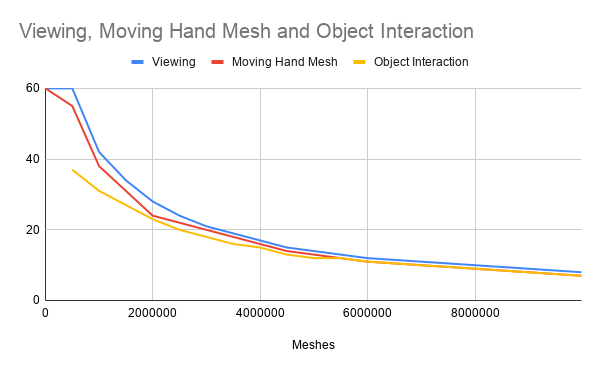
\includegraphics[width=0.45\textwidth]{fig/hololens2polycount}
    \caption{Figure showing frame rate as a function of polygon count on HoloLens 2. \\ Credit: \href{https://community.fologram.com/t/hololens-2-polygon-count-and-frame-rate/49}{Fologram}}
    \vspace{20pt}
    \label{fig:polycount}
\end{wrapfigure}

The first phase of development started by acquiring the surface model of the WHS rat brain created by \citet{Elden2017}. This was done by simply moving the FBX files from the \nameref{chap:vrvis} application and to a new Unity project. After initializing MRTK by following their \href{https://microsoft.github.io/MixedRealityToolkit-Unity/version/releases/2.2.0/Documentation/GettingStartedWithTheMRTK.html}{Getting Started documentation}, the application was ready to deploy on the HoloLens 2. This resulted in a barely running application as the polygon count of the brain model was orders of magnitude larger than what is recommended to maintain adequate performance on the HoloLens 2, which is in the order of 100,000 polygons shown in \autoref{fig:polycount}. The model used by Elden was scaled to run on workstation computer outputting to an HTC Vive, and thus his model was reduced from a original 16 million polygons to around 3 million. The HoloLens 2 runs all calculations on-device on a mobile ARM-based processing unit and naturally the brain model created for rendering on a dedicated workstation graphics card had to be further scaled down. 
This downscaling was first experimented with doing at run-time dynamically on-device using the library \textit{UnityMeshSimplifier}. It was quickly determined that this was not a viable solution both because of untenable processing time, but also because the simplified result had a huge impact on quality of model, hinting at the performance optimization that had to be done on the simplifier algorithm to be able to execute at run-time. The next and final solution for downscaling was to use the \textit{decimate} modifier in \nameref{chap:blender}. \textit{Incremental decimation} is a mesh simplification algorithm which trades some speed for higher mesh quality, in contrast to the \textit{vertex clustering} presumably used in UnityMeshSimplifier which prioritizes speed in such a way that topology is not preserved. Within Blender functionality for simple application of the modifier to all objects in a tree-structure was not found, or understood to exist, so a script applying the decimate modifier with a given ratio was written, see \autoref{item:blenderscript}. The \texttt{ratio} parameter is a value between 0 and 1, representing the scaling of the resulting mesh' polygon count.

\begin{lstlisting}[language=python, label={item:blenderscript}, caption={Blender script applying a decimate modifier to all relevant objects in a scene.}]
import bpy # importing the blender python library

def decimate(ratio, replace = True):
    # Finds all objects and filters irrelevant objects from the FBX 
    brainparts = [n for n in bpy.data.objects \
        if n.name not in ("Camera", "Light")] 

    for part in brainparts:
        mod = part.modifiers.new(type='DECIMATE', name='Decimate')
        mod.decimate_type = 'COLLAPSE'
        # Sets the specifies strength to the decimate operation. 
        mod.ratio = ratio
# Calls function with given decimate strength.
decimate(0.08)
\end{lstlisting}

The resulting decimated model, even at the ratio of 0.08, was visibly nearly indistinguishable from the original model when looking at them through the HoloLens 2 display which, as described in \autoref{chap:hololens2}, is somewhat blurry. \autoref{fig:decimate} shows the difference as seen in the Unity editor. Ultimately, a decimation ratio of 0.08 was chosen as a compromise between detail and performance being about 300,000 polygons, this compromise will be discussed further in \autoref{chap:discussperformance}. At this stage requirement 1 and 2 in the initial requirements from \autoref{chap:req} could conclusively be answer as possible and completed.
\begin{figure}[ht]
    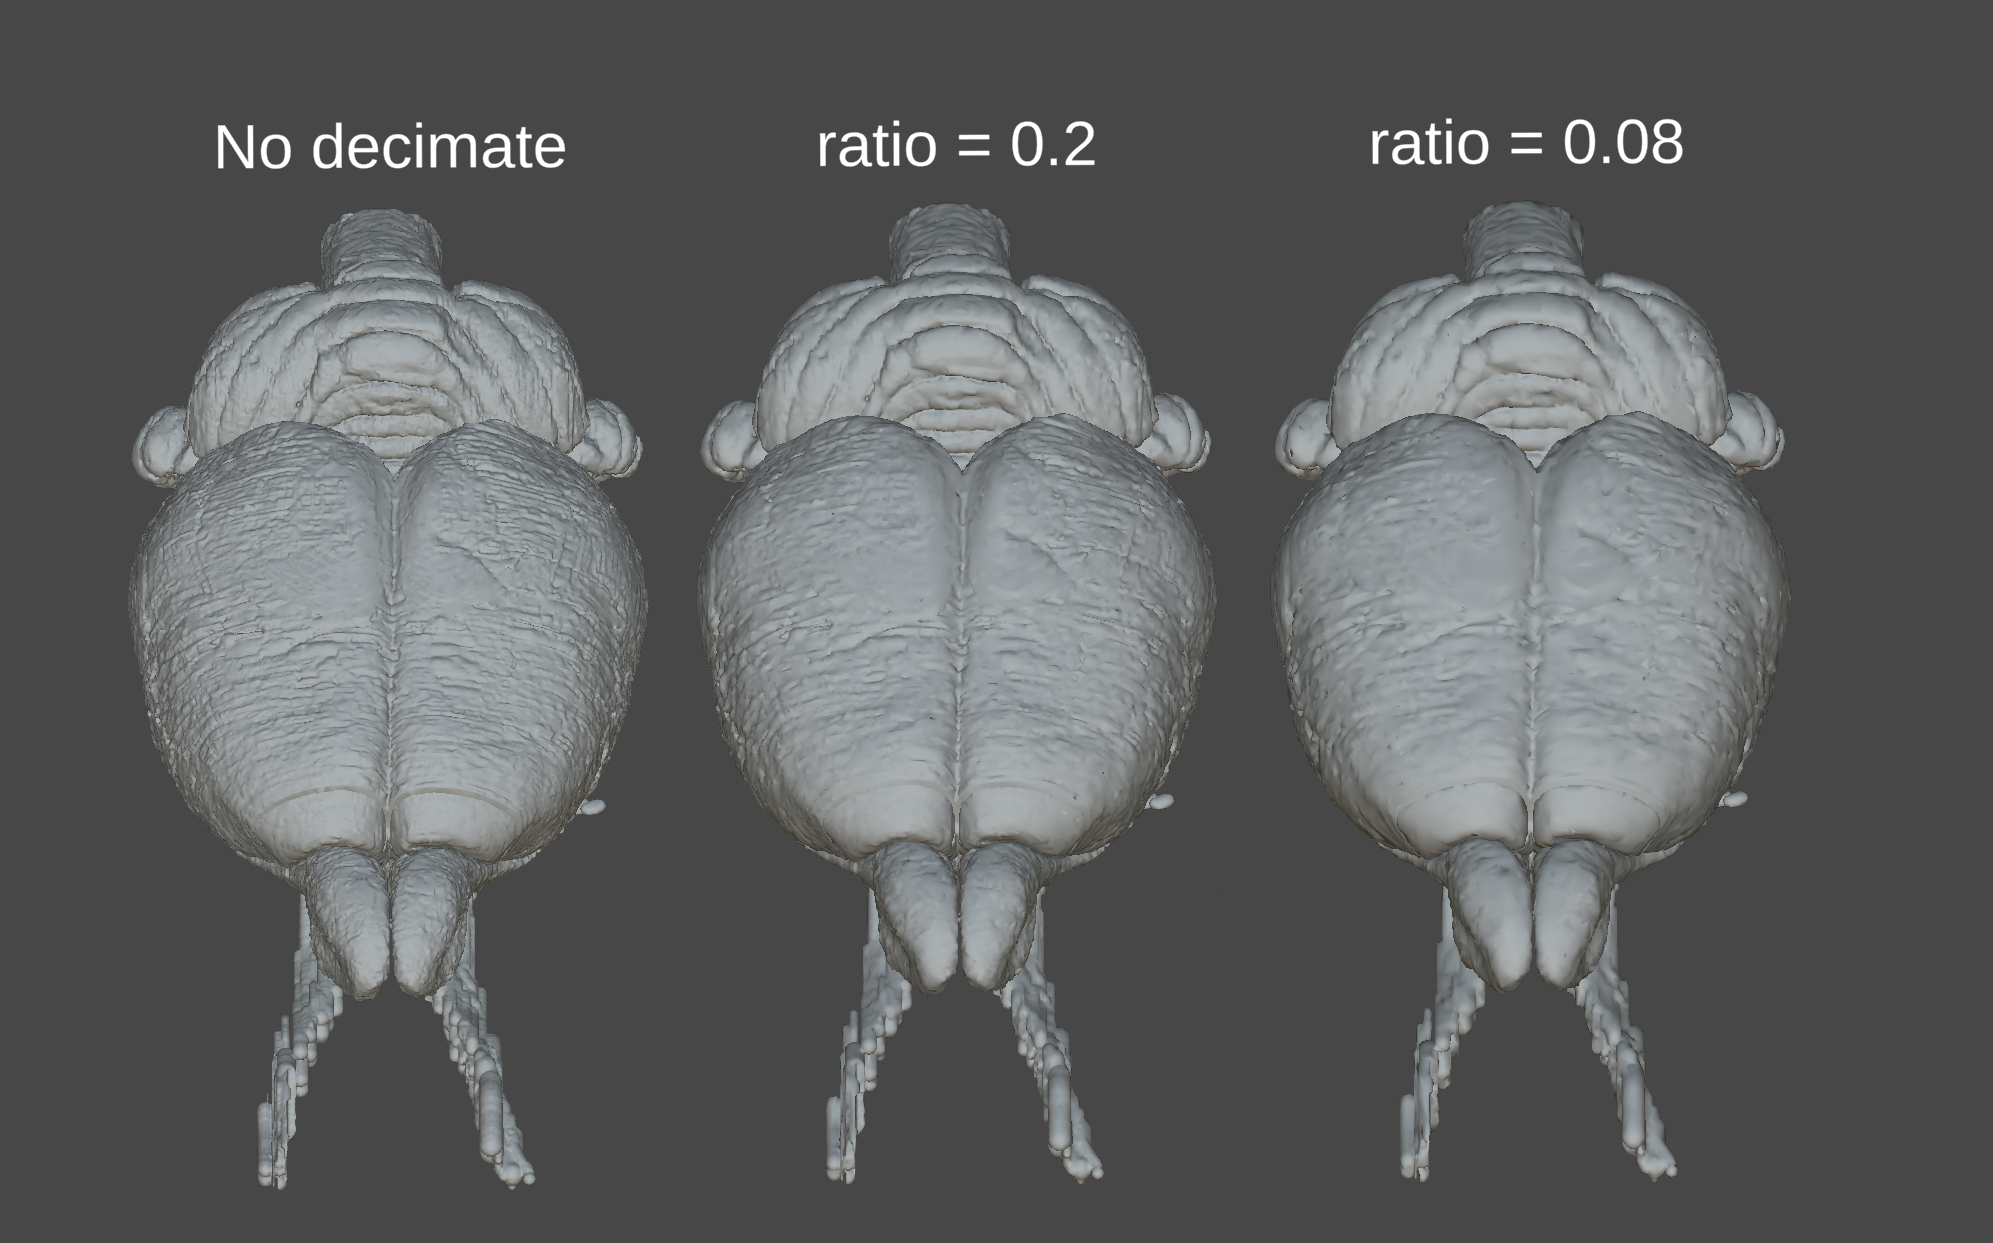
\includegraphics[width=\textwidth]{fig/brainmodeldecimateratio2.png}
    \caption{WHS rat brain models with decreasing polygon count.}
    \label{fig:decimate}
\end{figure}



\subsection*{First phase}
Having a surface model of the brain running reasonably well on the HoloLens 2, the next step in developing the application was to implement basic AR-based interact features. The brain model consist of an empty parent object with 29 children each containing the mesh of a delineated brain structure, see \autoref{fig:brainunitytree}. Adding the \texttt{Object Manipulator} component from MRTK and a standard Unity \texttt{Mesh Collider} component to each child in the brain model allows for picking apart the brain. This is done by grabbing and moving each separate structure with a MRTK defined \textit{pointer}, this is the logical abstraction for the simplest interact handling with HoloLens 2 giving the user a virtual laser pointer from their finger. The resulting action can be seen in \autoref{fig:grabbrain}. 

% \begin{wrapfigure}{r}{0.38\textwidth} 
%     \centering
%     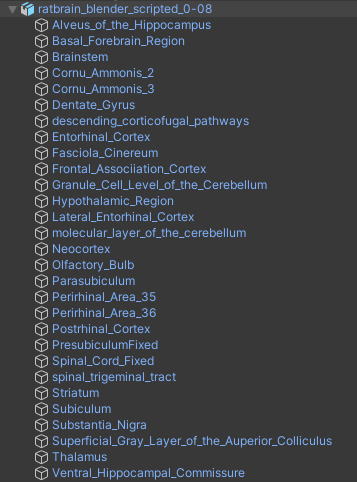
\includegraphics[width=0.35\textwidth]{fig/brainunitytree.png}
%     \caption{The tree structure of the Unity \texttt{GameObject} of the brain model.}
%     \vspace{-10pt}
%     \label{fig:brainunitytree}
% \end{wrapfigure}

\begin{figure}[ht]
    \centering
    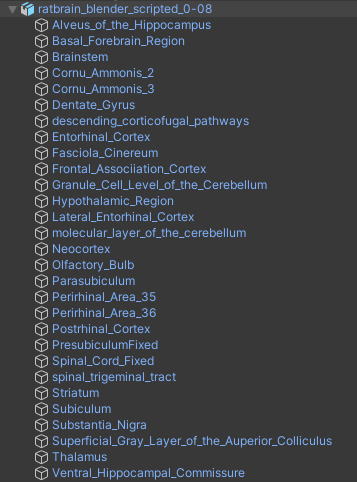
\includegraphics[width=0.30\textwidth]{fig/brainunitytree.png}
    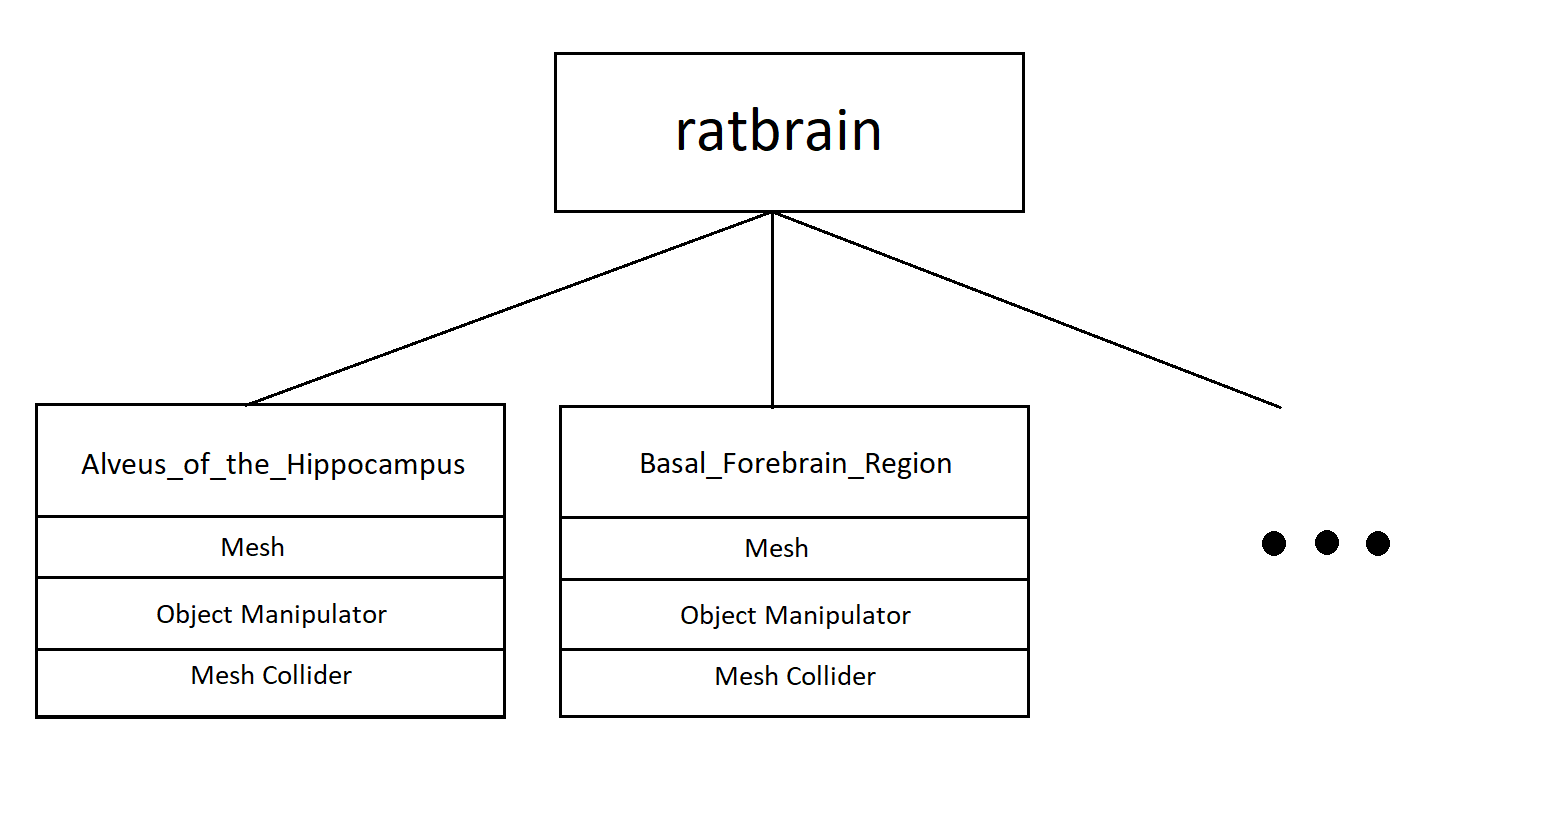
\includegraphics[width=0.60\textwidth]{fig/shittyassbraintreediagram.png}
    \caption{The tree structure of the Unity \texttt{GameObject} of the brain model.}
    \label{fig:brainunitytree}
\end{figure}

\begin{figure}[ht]
    \centering
    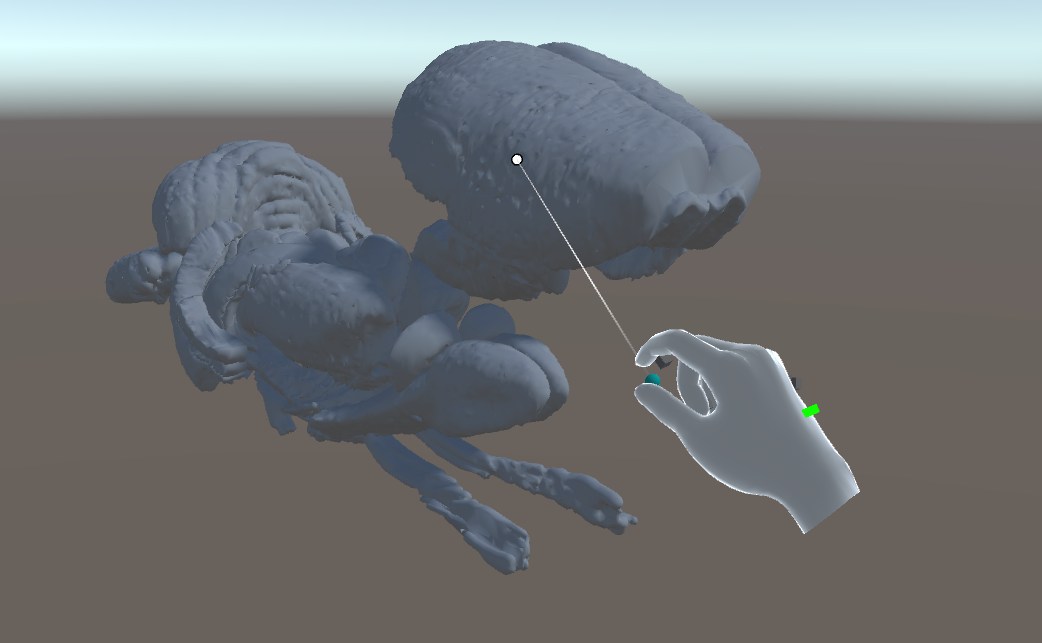
\includegraphics[width=0.8\textwidth]{fig/grabbrainsection.png}
    \caption{Grabbing the neocortex brain structure with a MRTK pointer in the Unity editor.}
    \label{fig:grabbrain}
\end{figure}

An apparent problem at this stage was that thought the brain structures are separate objects, they were difficult to visually distinguish from each other. A script which took all child objects and applied a random color to each was written and placed on the parent object, thus quickly giving some visual separation of the structures. While implementing this feature, the \textit{material} of each child was changed from Unity's default material to a \textit{MRTK Standard} material. Materials are the way Unity handles rendering details for each object, this is where shader, texture and general rendering options are configured. The MRTK Standard materials is a set of materials using the the \texttt{MixedRealityStandard.shader} shader, this shader is optimized for MR use, and superficially for HoloLens, and is meant for fulfill all shader-needs when developing for these platforms. 

With a colorful and manipulatable brain, the next natural step was tackling the system requirements, specifically the first functional requirement, implementing brain dissection. This was done with the clipping feature in the aforementioned MixedRealityStandard shader. Clipping has the effect of removing vertices by some defined function, and by using a prebuilt clipping plane prefab and declare on which meshes is should act, a dissection affect was created. A handle for manipulating the plane was added for ease of use, by dragged a ball the plane would move such that it was a fixed distance from the ball and perpendicular to the line between the ball and the center of the brain.

Further, a hovering menu displaying the name of the last grabbed brain structure and buttons for the actions moving, transparency and dissection was implemented. This was created by modifying a MRTK prefab and updating its name based on the name of the \texttt{GameObject} the \texttt{pointer} targeted while dragging, at the same time a selection lighting effect as applied by simply enabling \texttt{Border Lighting} in the MixedRealityStandard shader. Unity's layer functionality was used to ensure that it was a brain structurer being dragged. One last feature implemented at this phase was a tap-to-spawn feature, this entailed using the \texttt{pointer} to tap on the physical space, and using spatial awareness to place the brain at the locations the the user tapped. In MRTK spatial awareness is enabled by default and its mesh can be identified by a predefined Unity layer, thus \autoref{item:sudopointer} shows a simplified implementation of the \texttt{EventHandler} method, \texttt{OnPointerDown} which spawns the brain if the pointer is hitting the spatial awareness mesh and enables border lighting and menu text if it hits a brain structure.

\begin{lstlisting}[language=c, label={item:sudopointer}, caption={A simplified version of the event function called when a \texttt{Ponter} is clicked.}]
    void OnPointerDown(MixedRealityPointerEventData eventData)
    {
        if (!HasTarget(eventData.Pointer)) 
            return;
        Vector3 hitPoint = GetHitPoint(eventData.Pointer);
        GameObject target = GetCurrentTarget(eventData.Pointer);

        switch (target.layer)
        {
            case SpatialAwarenessLayer:
            {
                if (BrainHasNotBeenSpawned())
                    SpawnBrainAt(hitPoint);
            }
            case BrainStructureLayer:
            {
                if (selectedStructure != null)
                    DisableBorderLighting(selectedStructure);
                EnableBorderLighting(target);
                SetMenuText(target.name);
                selectedStructure = target;
            }
        }
    }
\end{lstlisting}

The application was deployed for HoloLens 2, and was a first MVP demo of the research project. \autoref{fig:mvpdemo} shows spawning of the brain model from image 1 to image 2 in the top row, notice the pointer on the table in image 1. Image 3 illustrates the clipping feature, while image 4 has a user taking out the \textit{cornu ammonis 3} brain structure.

\begin{figure}[h]
    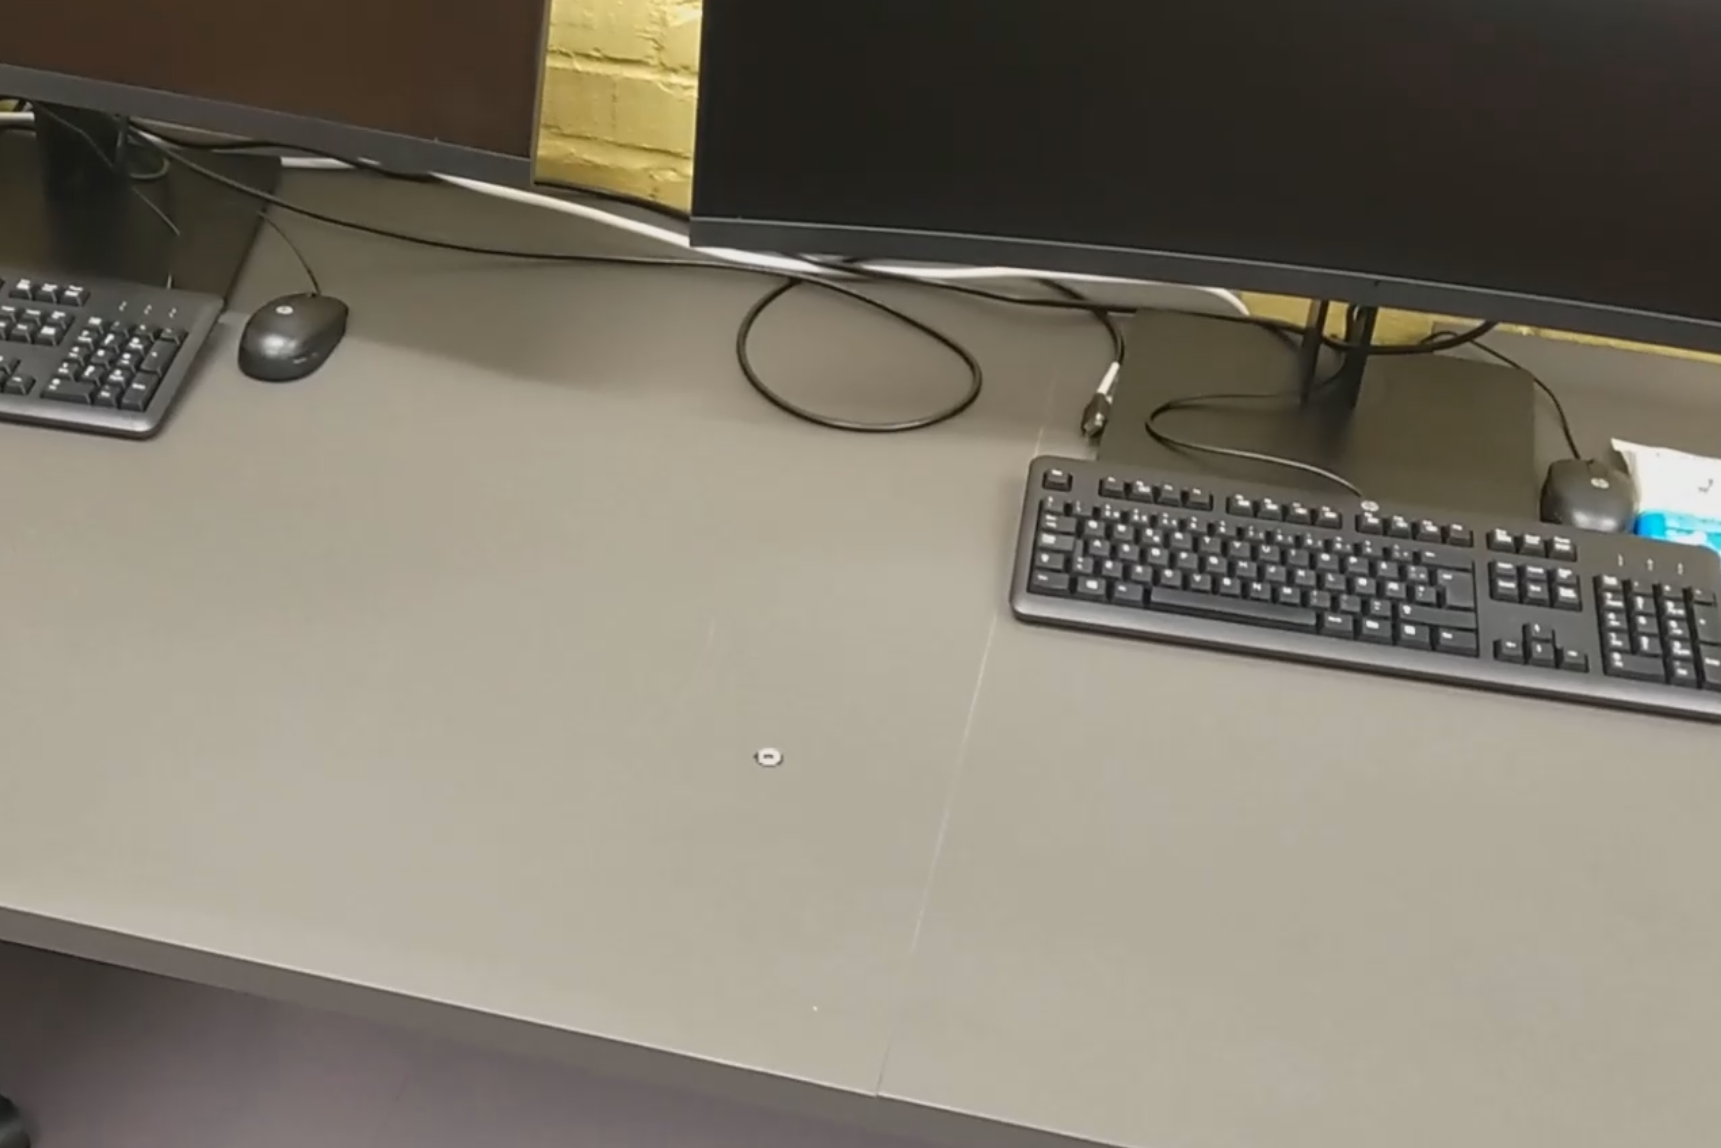
\includegraphics[width=0.5\textwidth]{fig/mvpdemo1.png}
    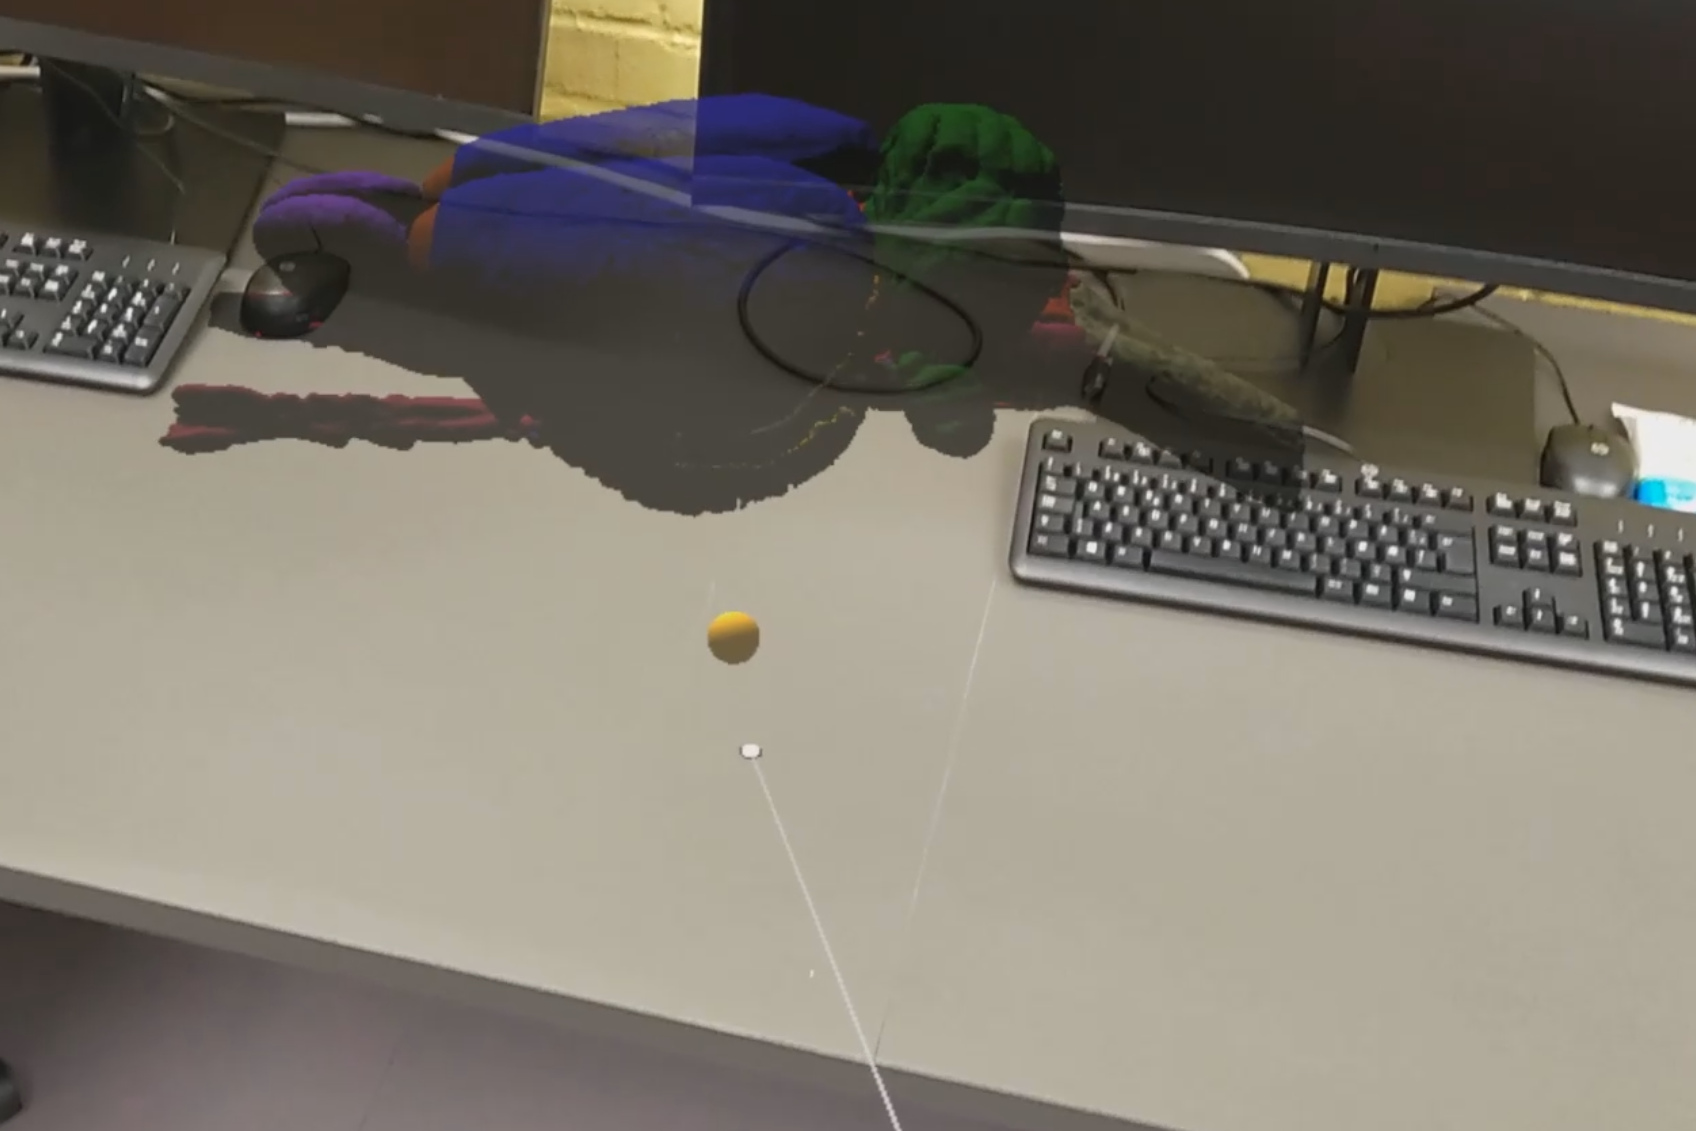
\includegraphics[width=0.5\textwidth]{fig/mvpdemo2.png}
    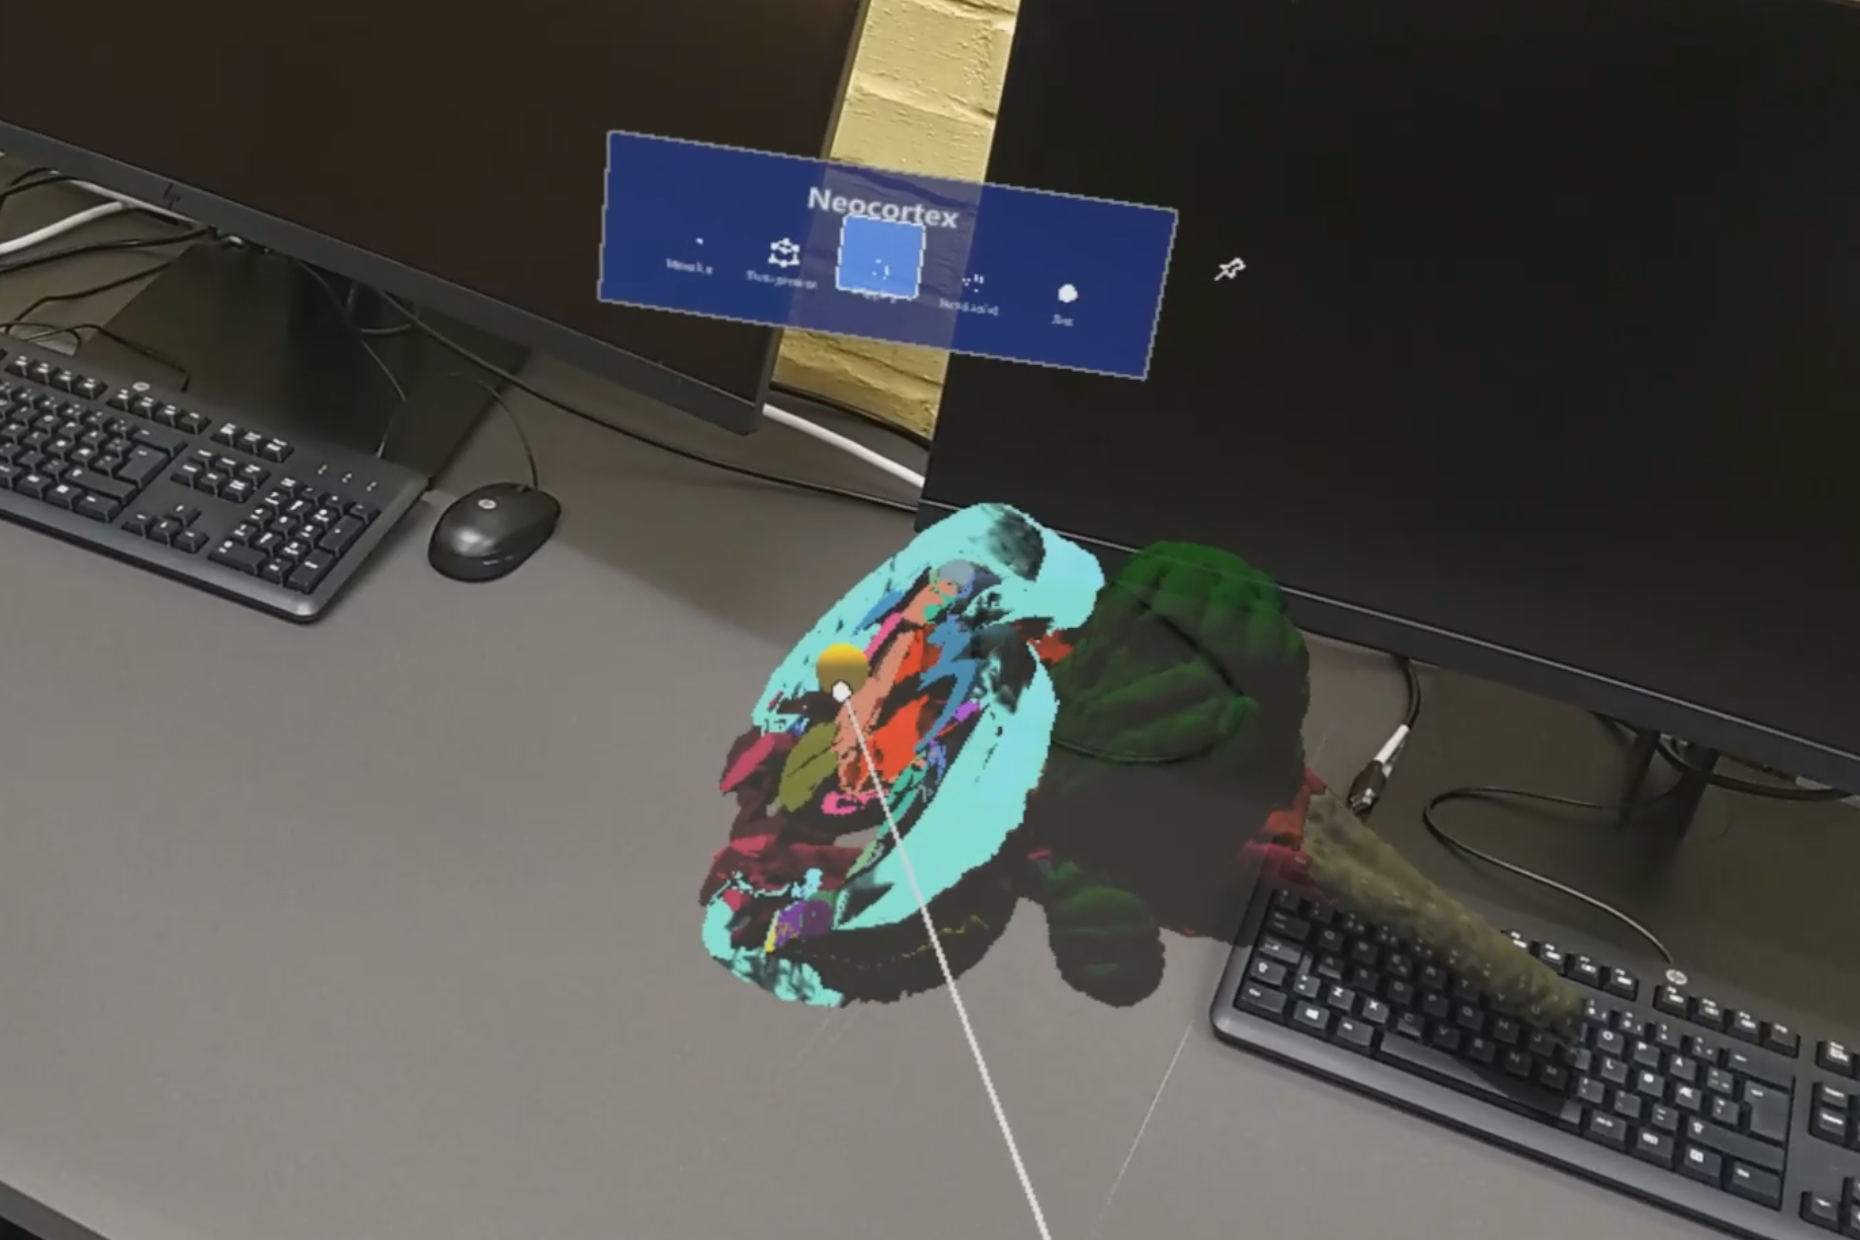
\includegraphics[width=0.5\textwidth]{fig/mvpdemo3.png}
    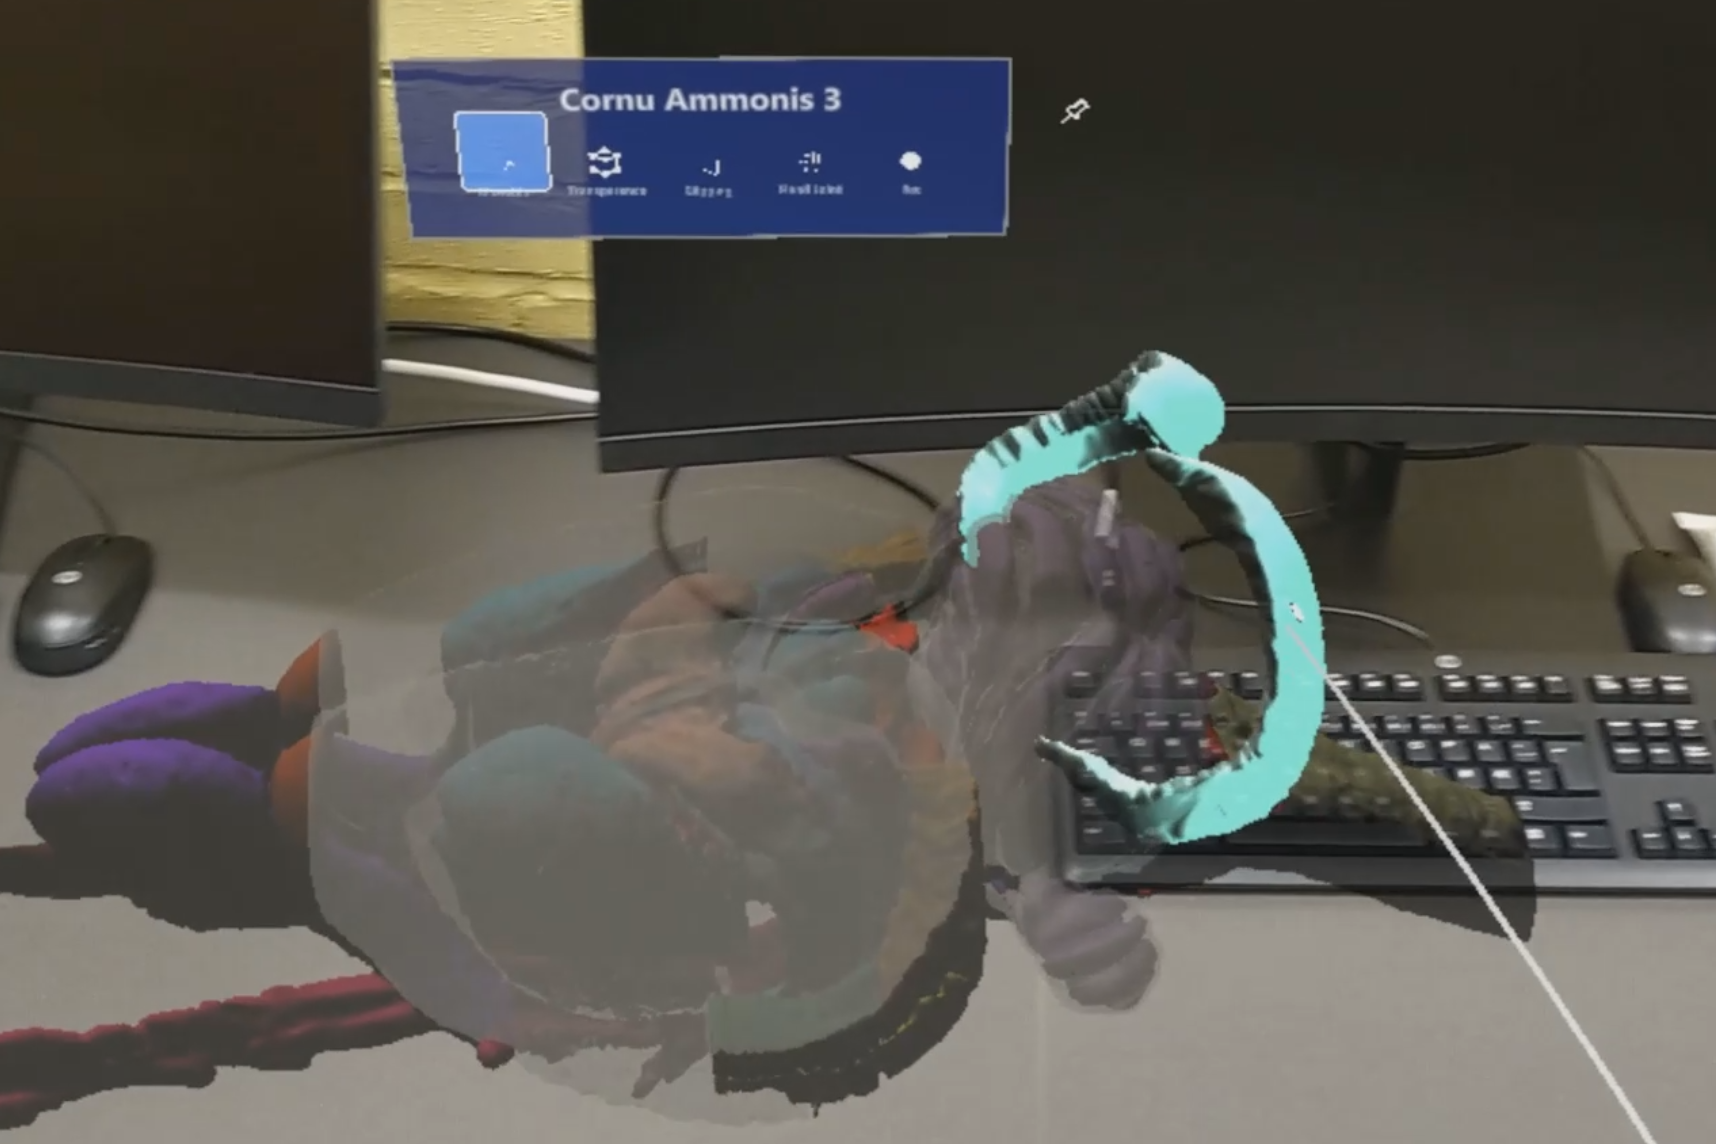
\includegraphics[width=0.5\textwidth]{fig/mvpdemo4.png}
    \caption{The first demo of the application.}
    \label{fig:mvpdemo}
\end{figure}




\subsection*{Porting to Android}
The application was originally developed for HoloLens 2, but other platforms were always in mind and because of the use of \nameref{chap:mrtk}, deploying to other platform was relatively easy, within the documentation for MRTK, there was guides for how to build for Android. Interaction on Android is more complicated though. Because all interaction happens on screen additional effort has to be laid down to implement a good user experience on smartphone.  







